\begin{enumerate}
	\item Заполните пропуски в таблице:
	\begin{figure*}[ht]
		\centering
		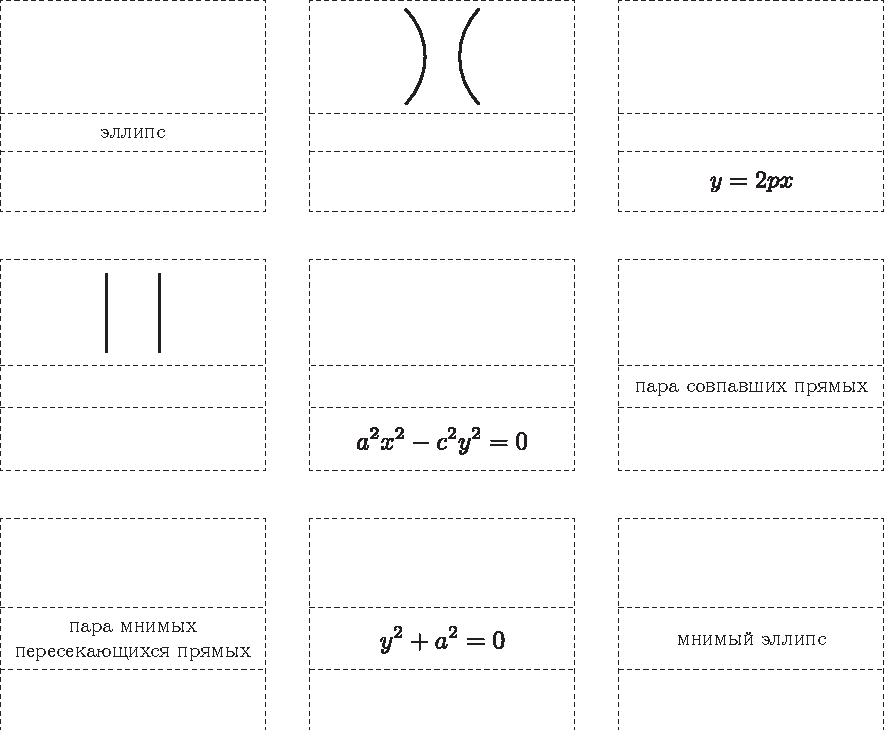
\includegraphics{1}
	\end{figure*}
	
	\item Какие замены переменных являются допустимыми при приведении кривой к каноническому виду?
	\begin{tasks}(2)
		\task $x' = 7x$	
		\task $x' = x + \sqrt{12}$
		\task $x' = x - y/2$,
		
		 	  $y' = x/2 + y$
		\task $x' = 3x/5 - 4y/5$,
	
		$y' = 4x/5 + 3y/5$

	\end{tasks}
	
	\item Запишите уравнения директрис для эллипса с $a=4$, $c=2$.
	\newpage
	\item Сформулируйте оптическое свойство эллипса (достаточно рисунка)
	\vspace{5cm}
	\item Эллипс задан уравнением $\frac{x^2}{1} + \frac{y^2}{4} = 9$. Найдите сумму расстояний от точки $M(\sqrt{8}, 2)$ до фокусов эллипса.

\end{enumerate}